%%%%%%%%%%%%%%%%%%%%%%%%%%%%%%%%%%%%%%%%%
% Beamer Presentation
% LaTeX Template
% Version 1.0 (10/11/12)
%
% This template has been downloaded from:
% http://www.LaTeXTemplates.com
%
% License:
% CC BY-NC-SA 3.0 (http://creativecommons.org/licenses/by-nc-sa/3.0/)
%
%%%%%%%%%%%%%%%%%%%%%%%%%%%%%%%%%%%%%%%%%

%----------------------------------------------------------------------------------------
%	PACKAGES AND THEMES
%----------------------------------------------------------------------------------------

\documentclass{beamer}

\mode<presentation> {

% The Beamer class comes with a number of default slide themes
% which change the colors and layouts of slides. Below this is a list
% of all the themes, uncomment each in turn to see what they look like.

%\usetheme{default}
%\usetheme{AnnArbor}
%\usetheme{Antibes}
%\usetheme{Bergen}
%\usetheme{Berkeley}
%\usetheme{Berlin}
%\usetheme{Boadilla}
%\usetheme{CambridgeUS}
%\usetheme{Copenhagen}
%\usetheme{Darmstadt}
%\usetheme{Dresden}
%\usetheme{Frankfurt}
%\usetheme{Goettingen}
%\usetheme{Hannover}
%\usetheme{Ilmenau}
%\usetheme{JuanLesPins}
%\usetheme{Luebeck}
\usetheme{Madrid}
%\usetheme{Malmoe}
%\usetheme{Marburg}
%\usetheme{Montpellier}
%\usetheme{PaloAlto}
%\usetheme{Pittsburgh}
%\usetheme{Rochester}
%\usetheme{Singapore}
%\usetheme{Szeged}
%\usetheme{Warsaw}

% As well as themes, the Beamer class has a number of color themes
% for any slide theme. Uncomment each of these in turn to see how it
% changes the colors of your current slide theme.

%\usecolortheme{albatross}
%\usecolortheme{beaver}
%\usecolortheme{beetle}
%\usecolortheme{crane}
%\usecolortheme{dolphin}
%\usecolortheme{dove}
%\usecolortheme{fly}
%\usecolortheme{lily}
%\usecolortheme{orchid}
%\usecolortheme{rose}
%\usecolortheme{seagull}
%\usecolortheme{seahorse}
%\usecolortheme{whale}
%\usecolortheme{wolverine}

%\setbeamertemplate{footline} % To remove the footer line in all slides uncomment this line
%\setbeamertemplate{footline}[page number] % To replace the footer line in all slides with a simple slide count uncomment this line

%\setbeamertemplate{navigation symbols}{} % To remove the navigation symbols from the bottom of all slides uncomment this line
}

\usepackage{graphicx} % Allows including images
\usepackage{booktabs} % Allows the use of \toprule, \midrule and \bottomrule in tables
\usepackage{listings}
\usepackage{color}
\usepackage{ulem}
\usepackage{array}

\definecolor{mygreen}{rgb}{0,0.6,0}
\definecolor{mygray}{rgb}{0.5,0.5,0.5}
\definecolor{mymauve}{rgb}{0.58,0,0.82}

\lstset{ %
  backgroundcolor=\color{white},   % choose the background color; you must add \usepackage{color} or \usepackage{xcolor}
  basicstyle=\scriptsize,        % the size of the fonts that are used for the code
  breakatwhitespace=false,         % sets if automatic breaks should only happen at whitespace
  breaklines=true,                 % sets automatic line breaking
  captionpos=b,                    % sets the caption-position to bottom
  commentstyle=\color{mygreen},    % comment style
  deletekeywords={...},            % if you want to delete keywords from the given language
  escapeinside={\%*}{*)},          % if you want to add LaTeX within your code
  extendedchars=true,              % lets you use non-ASCII characters; for 8-bits encodings only, does not work with UTF-8
%  frame=single,                    % adds a frame around the code
  keepspaces=true,                 % keeps spaces in text, useful for keeping indentation of code (possibly needs columns=flexible)
  keywordstyle=\color{blue},       % keyword style
  language=Octave,                 % the language of the code
  morekeywords={*,...},            % if you want to add more keywords to the set
  numbers=none,                    % where to put the line-numbers; possible values are (none, left, right)
  numbersep=5pt,                   % how far the line-numbers are from the code
  numberstyle=\tiny\color{mygray}, % the style that is used for the line-numbers
  %rulecolor=\color{black},         % if not set, the frame-color may be changed on line-breaks within not-black text (e.g. comments (green here))
  showspaces=false,                % show spaces everywhere adding particular underscores; it overrides 'showstringspaces'
  showstringspaces=false,          % underline spaces within strings only
  showtabs=false,                  % show tabs within strings adding particular underscores
  stepnumber=2,                    % the step between two line-numbers. If it's 1, each line will be numbered
  stringstyle=\color{mymauve},     % string literal style
  tabsize=2,                       % sets default tabsize to 2 spaces
  title=\lstname                   % show the filename of files included with \lstinputlisting; also try caption instead of title
}

%\lstset{escapechar=@,style=customc}

%----------------------------------------------------------------------------------------
%	TITLE PAGE
%----------------------------------------------------------------------------------------

\title[RdfLiveNews]{RdfLiveNews\newline --- \newline Real-time RDF Extraction from\newline Unstructured Data Streams}

\author{Daniel Gerber, Sebastian Hellmann, Lorenz Bühmann, Tommaso Soru, Ricardo Usbeck and Axel-Cyrille Ngonga Ngomo} % Your name
\institute[AKSW] % Your institution as it will appear on the bottom of every slide, may be shorthand to save space
{
University of Leipzig \\ % Your institution for the title page
\medskip
\textit{ngonga@informatik.uni-leipzig.de} % Your email address
}
\date{October 24th, 2013} % Date, can be changed to a custom date

\begin{document}

\begin{frame}
\titlepage % Print the title page as the first slide
\end{frame}

%\begin{frame}
%\frametitle{Overview} % Table of contents slide, comment this block out to remove it
%\tableofcontents % Throughout your presentation, if you choose to use \section{} and \subsection{} commands, these will automatically be printed on this slide as an overview of your presentation
%\end{frame}
\begin{frame}{Motivation}
	\begin{columns}[c]
		\column{.5\textwidth}
			\centering
			\begin{enumerate}
				\item 60\% of LD is static
				\item Most data is encyclopedic
				\begin{itemize}
					\item LinkedTCGA (7.6 $\times 10^9$ T)
					\item LinkedGeoData ($10^9$ T)
					\item ...
				\end{itemize}
				\item Lack of actuality
				\item Live tools gather data from semi-structured data
			\end{enumerate}
		\column{.5\textwidth}
			\centering
			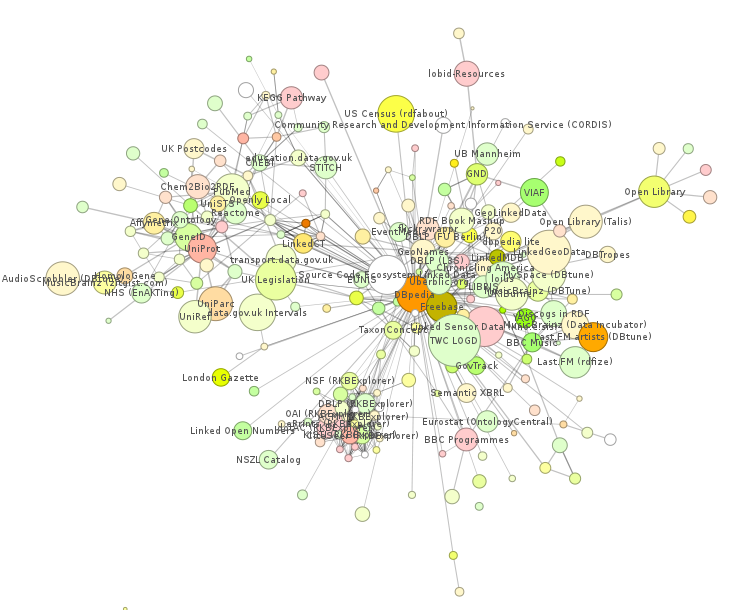
\includegraphics[width=\textwidth]{../images/opendata_graph}
	\end{columns}
\pause
\begin{alertblock}{Goal}
Provide actual data in RDF that allow  answering questions such as 
\texttt{Give me all news of the last week from the New York Times pertaining to the director of Nokia.}
\end{alertblock}

\end{frame}
%------------------------------------------------

\begin{frame}{Requirements}
\begin{columns}[c]
		\column{.7\textwidth}
    \begin{itemize}
        \item Timeliness needs to run 24/7 
        \item Has to handle large amounts of data
        \item Needs to able to handle unstructured data
        \item Extraction has to be precise
        \item Open information extraction
    \end{itemize}
 \column{.3\textwidth}

\includegraphics[width=\textwidth]{../images/question}
\end{columns}
\end{frame}

%------------------------------------------------

\begin{frame}
    \frametitle{Architecture}
    %\begin{block}{RdfLiveNews processing pipeline}
        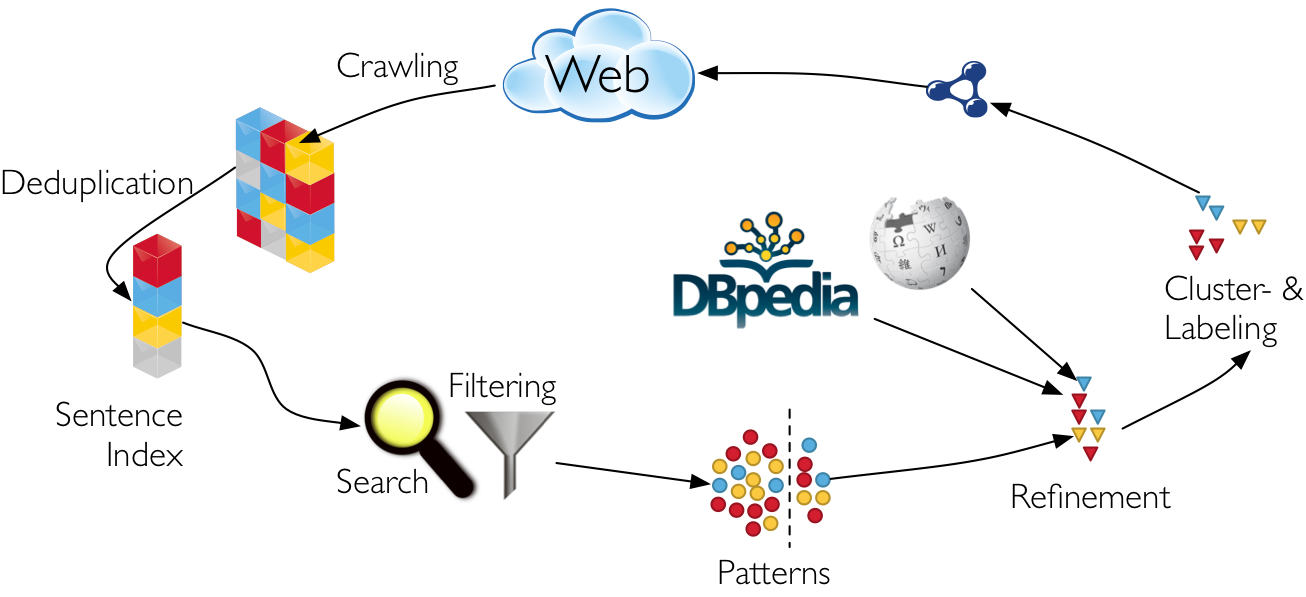
\includegraphics[width=\textwidth]{../images/rdflivenews_architecture.pdf}
    %\end{block}
\end{frame}

%------------------------------------------------

\begin{frame}
   \frametitle{Data Acquisition and Deduplication}
\begin{itemize}
\item Assumptions
  \begin{enumerate}
        \item Unstructured data source $S_i$ emits continuous data streams $D_i$ (e.g., RSS feeds)
        \item Each data stream $D_i$ consists of atomic elements $d^i_j$        
    \end{enumerate}
\pause
\item Approach
\begin{enumerate}
\item Gather all elements of $D_i$ emitted between $t$ and $t+d$ in $D^i_{[t,t+d]}$
\item Apply sentence splitting and use sentences as atoms for processing
\item Perform string-similarity-based deduplication
\end{enumerate}
\end{itemize}
\end{frame}

%------------------------------------------------

\begin{frame}
    \frametitle{Architecture}
    %\begin{block}{RdfLiveNews processing pipeline}
        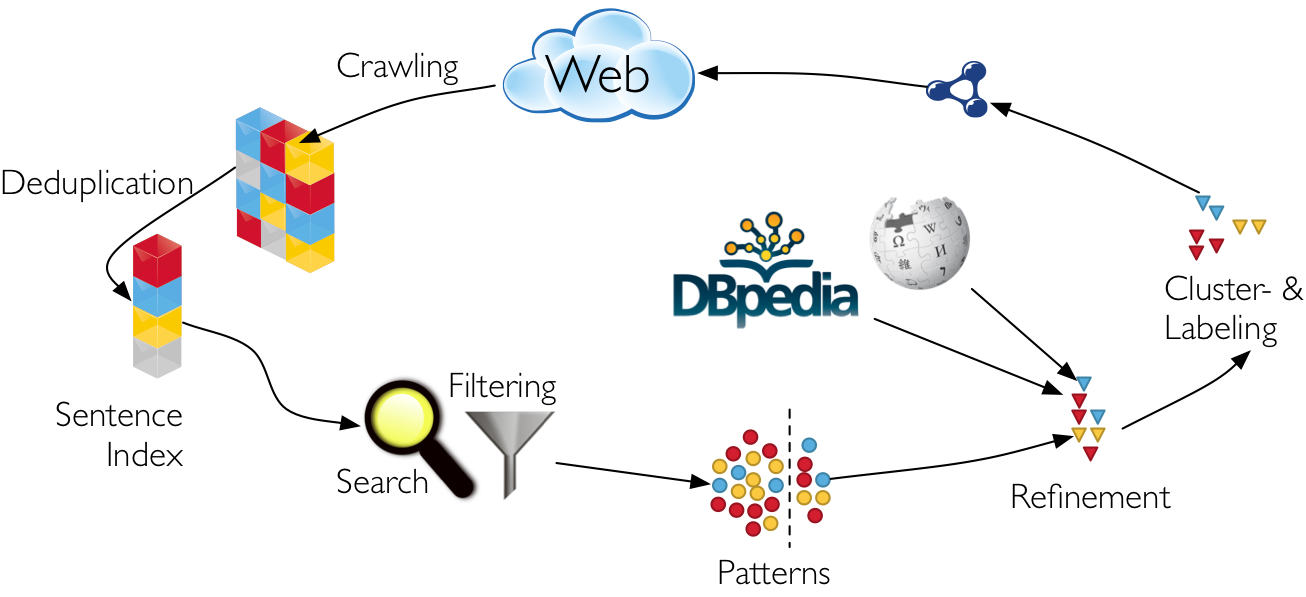
\includegraphics[width=\textwidth]{../images/rdflivenews_architecture.pdf}
    %\end{block}
\end{frame}

%------------------------------------------------

\begin{frame}
    \frametitle{Search \& Filtering}
    \begin{itemize}
        \item Apply Part Of Speech Tagging or Named Entity Recognition (Loc, Per, Org, Misc)
    \end{itemize}
    \begin{block}{POS Tagging}
    % hier steht nur Smith -> John Smith wird dann vervollständigt
        ... Smith/NNP ,/, is/VBZ the/DT manager/NN of/IN ABC/NNP.
    \end{block}
\pause
    \begin{block}{Example: Pattern}
        $p$ = ([, is the manager of], {(\textcolor{red}{John Smith}, ABC)})
    \end{block}
    \begin{itemize}
\item Patterns must
\begin{itemize}
        \item Contain a verb or noun, at least one non stop-word \& shorter than 50 characters
        \item Sort by number of elements in support set and take top n\%
    \end{itemize}
\item \textcolor{red}{Where does ``John'' come from?}
\end{itemize}
\end{frame}

%------------------------------------------------

\begin{frame}
    \frametitle{Pattern Refinement}

    \begin{itemize}
        \item Refine patterns by disambiguating support set to 
\begin{itemize}
        \item Complete entity names (``John Smith'')
\item Find suitable \textit{rdfs:range} \& \textit{rdfs:domain}
\end{itemize}
        \item Score each candidate URI based on 4 measures (local/global context, apriori \& string similarity)
        \item Use normalized and weighted features to find best URI or create new URI
        \item Use \textit{rdf:type}s of URIs in support set to find \textit{rdfs:domain/range}: \texttt{MostGeneric} vs. \texttt{MostSpecific}
    \end{itemize}
    \begin{block}{Example: Refined Pattern}
        $p_r$ = ([, is the manager of], {(John Smith \textless dbr:John\_Smith\textgreater, ABC \textless dbr:ABC\textgreater)}, dbo:Person, dbo:Company)
    \end{block}
\end{frame}
%------------------------------------------------

\begin{frame}
    \frametitle{Architecture}
    %\begin{block}{RdfLiveNews processing pipeline}
        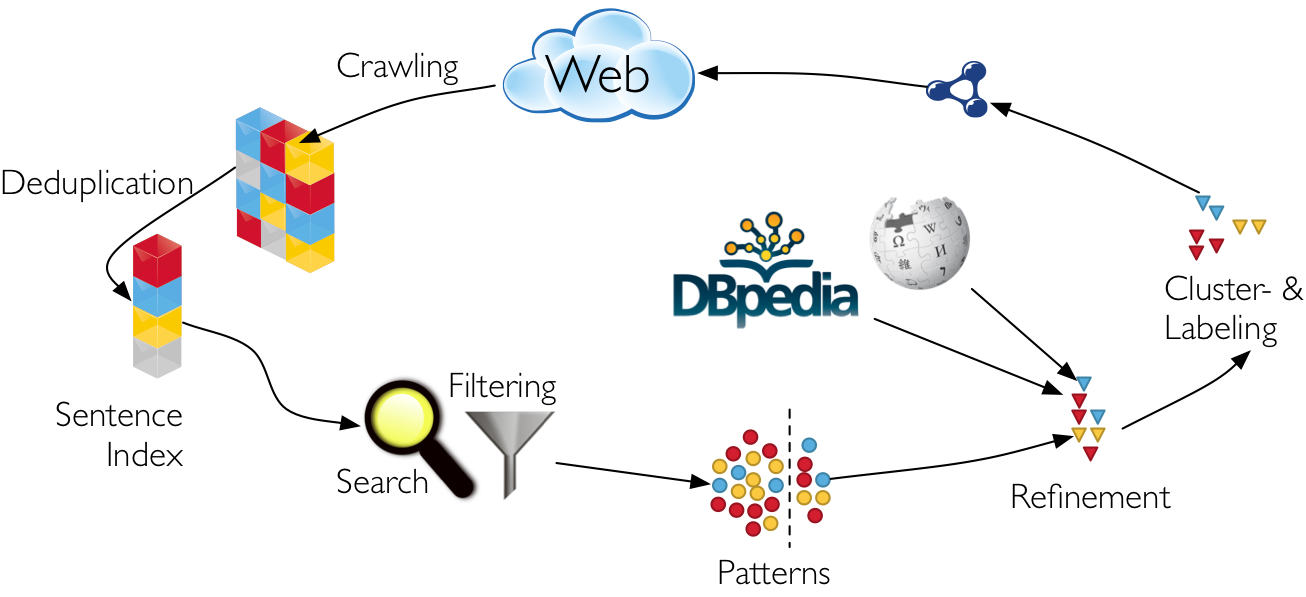
\includegraphics[width=\textwidth]{../images/rdflivenews_architecture.pdf}
    %\end{block}
\end{frame}


%------------------------------------------------

\begin{frame}
    \frametitle{Clustering \& Labeling}
\begin{block}{Idea}
\begin{itemize}
        \item Merge patterns to groups of patterns that express a certain relation
	\item Group of patterns stand for a predicate
\end{itemize}
\end{block}
\pause
    \begin{itemize}
        \item Baseline (string similarity) often fails, e.g., ``attorney'' vs. ``lawyer''
\pause
\item Approach
\begin{enumerate}
	\item Preprocess patterns by using lemmatization and stop word removal
        \item Use linear combination of Wordnet and string similarity  to generate similarity graph 
            %\begin{itemize}
              %  \item Filter stop-words
                %\item Apply lemmatization
                %\item Select maximum similarity score for all token combinations of two patterns
                %\item Combine string and wordnet similarity via linear combination
            %\end{itemize}
        \item Cluster using BorderFlow with hardening
        \item Majority vote to determine cluster labels
    \end{enumerate}
    \end{itemize}
    \begin{block}{Example: Clustering}
        sim([\sout{,} \sout{is}(be) \sout{the} manager \sout{of}], [\sout{,} \sout{was}(be) \sout{the} executive director \sout{of}]) = 0.8
    \end{block}
\end{frame}
%------------------------------------------------

\begin{frame}
    \frametitle{Architecture}
    %\begin{block}{RdfLiveNews processing pipeline}
        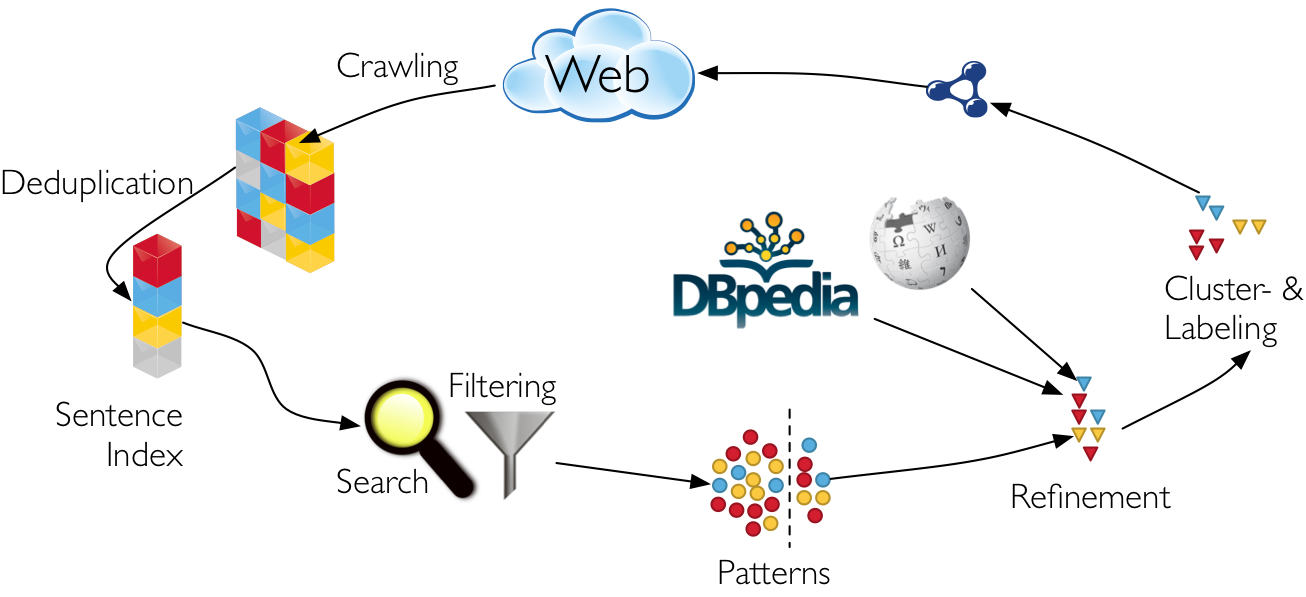
\includegraphics[width=\textwidth]{../images/rdflivenews_architecture.pdf}
    %\end{block}
\end{frame}


%------------------------------------------------

\begin{frame}
    \frametitle{RDF Generation}
    \begin{itemize}
        \item Facts and properties are mapped to RDF
        \item Metadata: extraction/publication date and provenance links to text
        \item Mint URIs to provide linked data
        %\item We use NIF (NLP Interchange Format)
        \item Link predicates to DBpedia via LIMES
    \end{itemize}
\end{frame}

%------------------------------------------------

\begin{frame}[fragile]
\frametitle{Example}
    \begin{lstlisting}
## cluster information
rlno:directorOf a owl:ObjectProperty ;skos:prefLabel "director of" ,
skos:altLabel ", director of " ;
owl:equivalentProperty dbp:director .

## extracted facts:
rlnr:Rolf_Heuer a dbo:Person; rdfs:label "Rolf Heuer"@en ;rlno:directorOf dbpedia:CERN .
dbpedia:CERN a owl:Thing ; rdfs:label "CERN"@en .

## provenance tracking with NIF:
<char=0,10> itsrdf:taClassRef dbo:Person ; itsrdf:taIdentRef rlnr:Rolf_Heuer .
<char=14,18> itsrdf:taIdentRef dbpedia:CERN .
<char=11,24> nif:anchorOf ", director of"^^xsd:string ;itsrdf:taPropRef rlno:directorOf .

## detailed NIF output with context, indices and anchorOf
<char=0,> a nif:String , nif:Context , nif:RFC5147String ;nif:isString "Rolf Heuer , director of CERN , said the newly discovered particle is a boson .... - an extremely fine distinction." ;
nif:sourceUrl <http://www.necn.com/07/04/12/Scientists-discover-new-subatomic-partic/landing.html?blockID=735470&feedID=4213>;
\end{lstlistings}
    \end{lstlisting}

\end{frame}

%------------------------------------------------

\begin{frame}
    \frametitle{Experiments}
    \begin{enumerate}
        \item How good is the RDFLiveNews URI disambiguation? 
        \item Can we find clusters of similar patterns? 
        \item Which quality does the generated RDF have? 
        \item Is near real-time RDF generation possible? 
    \end{enumerate}
\end{frame}

%------------------------------------------------

\begin{frame}
    \frametitle{Experimental Setup}
    \begin{itemize}
        \item Crawled 1457 RSS feeds for 76 hours 
        \item 38 time slices of 2 hours and 11.7M sentences = 100\% 
        \item Average number of sentences/article is about 26.5 
        \item Average number of articles/timeslice is about 3445 
        \item Two subsets: 10\% and 1\% 
    \end{itemize}
\end{frame}

%------------------------------------------------

\begin{frame}
    \frametitle{URI Disambiguation}
    \begin{itemize}
        \item Generated gold standard from 1\%, 473 entity pairs
        \item Hill climbing with random initialization
        %\item Precision: ratio between correctly found URIs to URIs above the threshold $\lambda$
        %\item Recall: ratio between number of correct URIs and the total number of URIs in the gold standard
        \item $P_{max} = 0.85$ / $R = 0.407$ / $F = 0.55$
        \item $F_{max} = 0.665$ / $P = 0.67$ / $R = 0.66$
        \item AIDA achieves $F = 0.6$%, 2min/article
    \end{itemize}
\end{frame}

%------------------------------------------------

\begin{frame}
    \frametitle{Pattern Clustering}
    \begin{itemize}
        \item Manually clustered patterns from gold standard 
        \item Sensitivity ($Se$, similar to recall)%: fraction of patterns of pattern mapping i which are found in cluster j 
        \item Positive Predictive Value ($PPV$, similar to precision)%: proportion of members of cluster j which belong to pattern mapping i, relative to the total number of members of this cluster assigned to all pattern mappings 
        \item Accuracy = $\sqrt{Se \times PPV}$
\pause

        \item Wordnet-String-Similarity: S = 0.712, PPV = 0.955, A = 0.825 
        \item String-Similarity: A = 0.691
	\item Wordnet-Similarity: A = 0.789 
    \end{itemize}
\end{frame}

%------------------------------------------------

\begin{frame}
    \frametitle{RDF Extraction}
    \begin{itemize}
	\item Random selection of 100 triples
        \item 5 different evaluation sets, each set may only contain properties of clusters with at least $i = 1 \dots 5$ patterns
    \end{itemize}
    \begin{table}
    \begin{tabular}{rccccc} 
        \toprule
		$E_i$               &  1       &  2       &  3       &  4       &    5      \\ \midrule
		$S_{Acc}$           &  0.81  &  0.88  &  0.86  &  0.857  &  0.804 \\ 
		$P_{Acc}$           &  0.86  &  0.89  &  0.90  &  0.935  &  1.00 \\ 
        $O_{Acc}$           &  0.93  &  0.91  &  0.90  &  0.948  &  0.941 \\ 
		$Total_{Acc}$       &  0.86  &  0.892  &  0.885  &  0.911  &  0.906 \\ 
		$|E_i|$             &  100     &  100     &  100     &  77      &  51 \\ 
		$|P| \in |E_i|$     &  28      &  22      &  12      &  6       &  1 \\ \bottomrule
    \end{tabular}
    \end{table}
\end{frame}

%------------------------------------------------

\begin{frame}
    \frametitle{Scalability}
    \begin{block}{Runtimes for different components and corpora (1\% left, 10\% middle, 100\% right) per iteration.}
        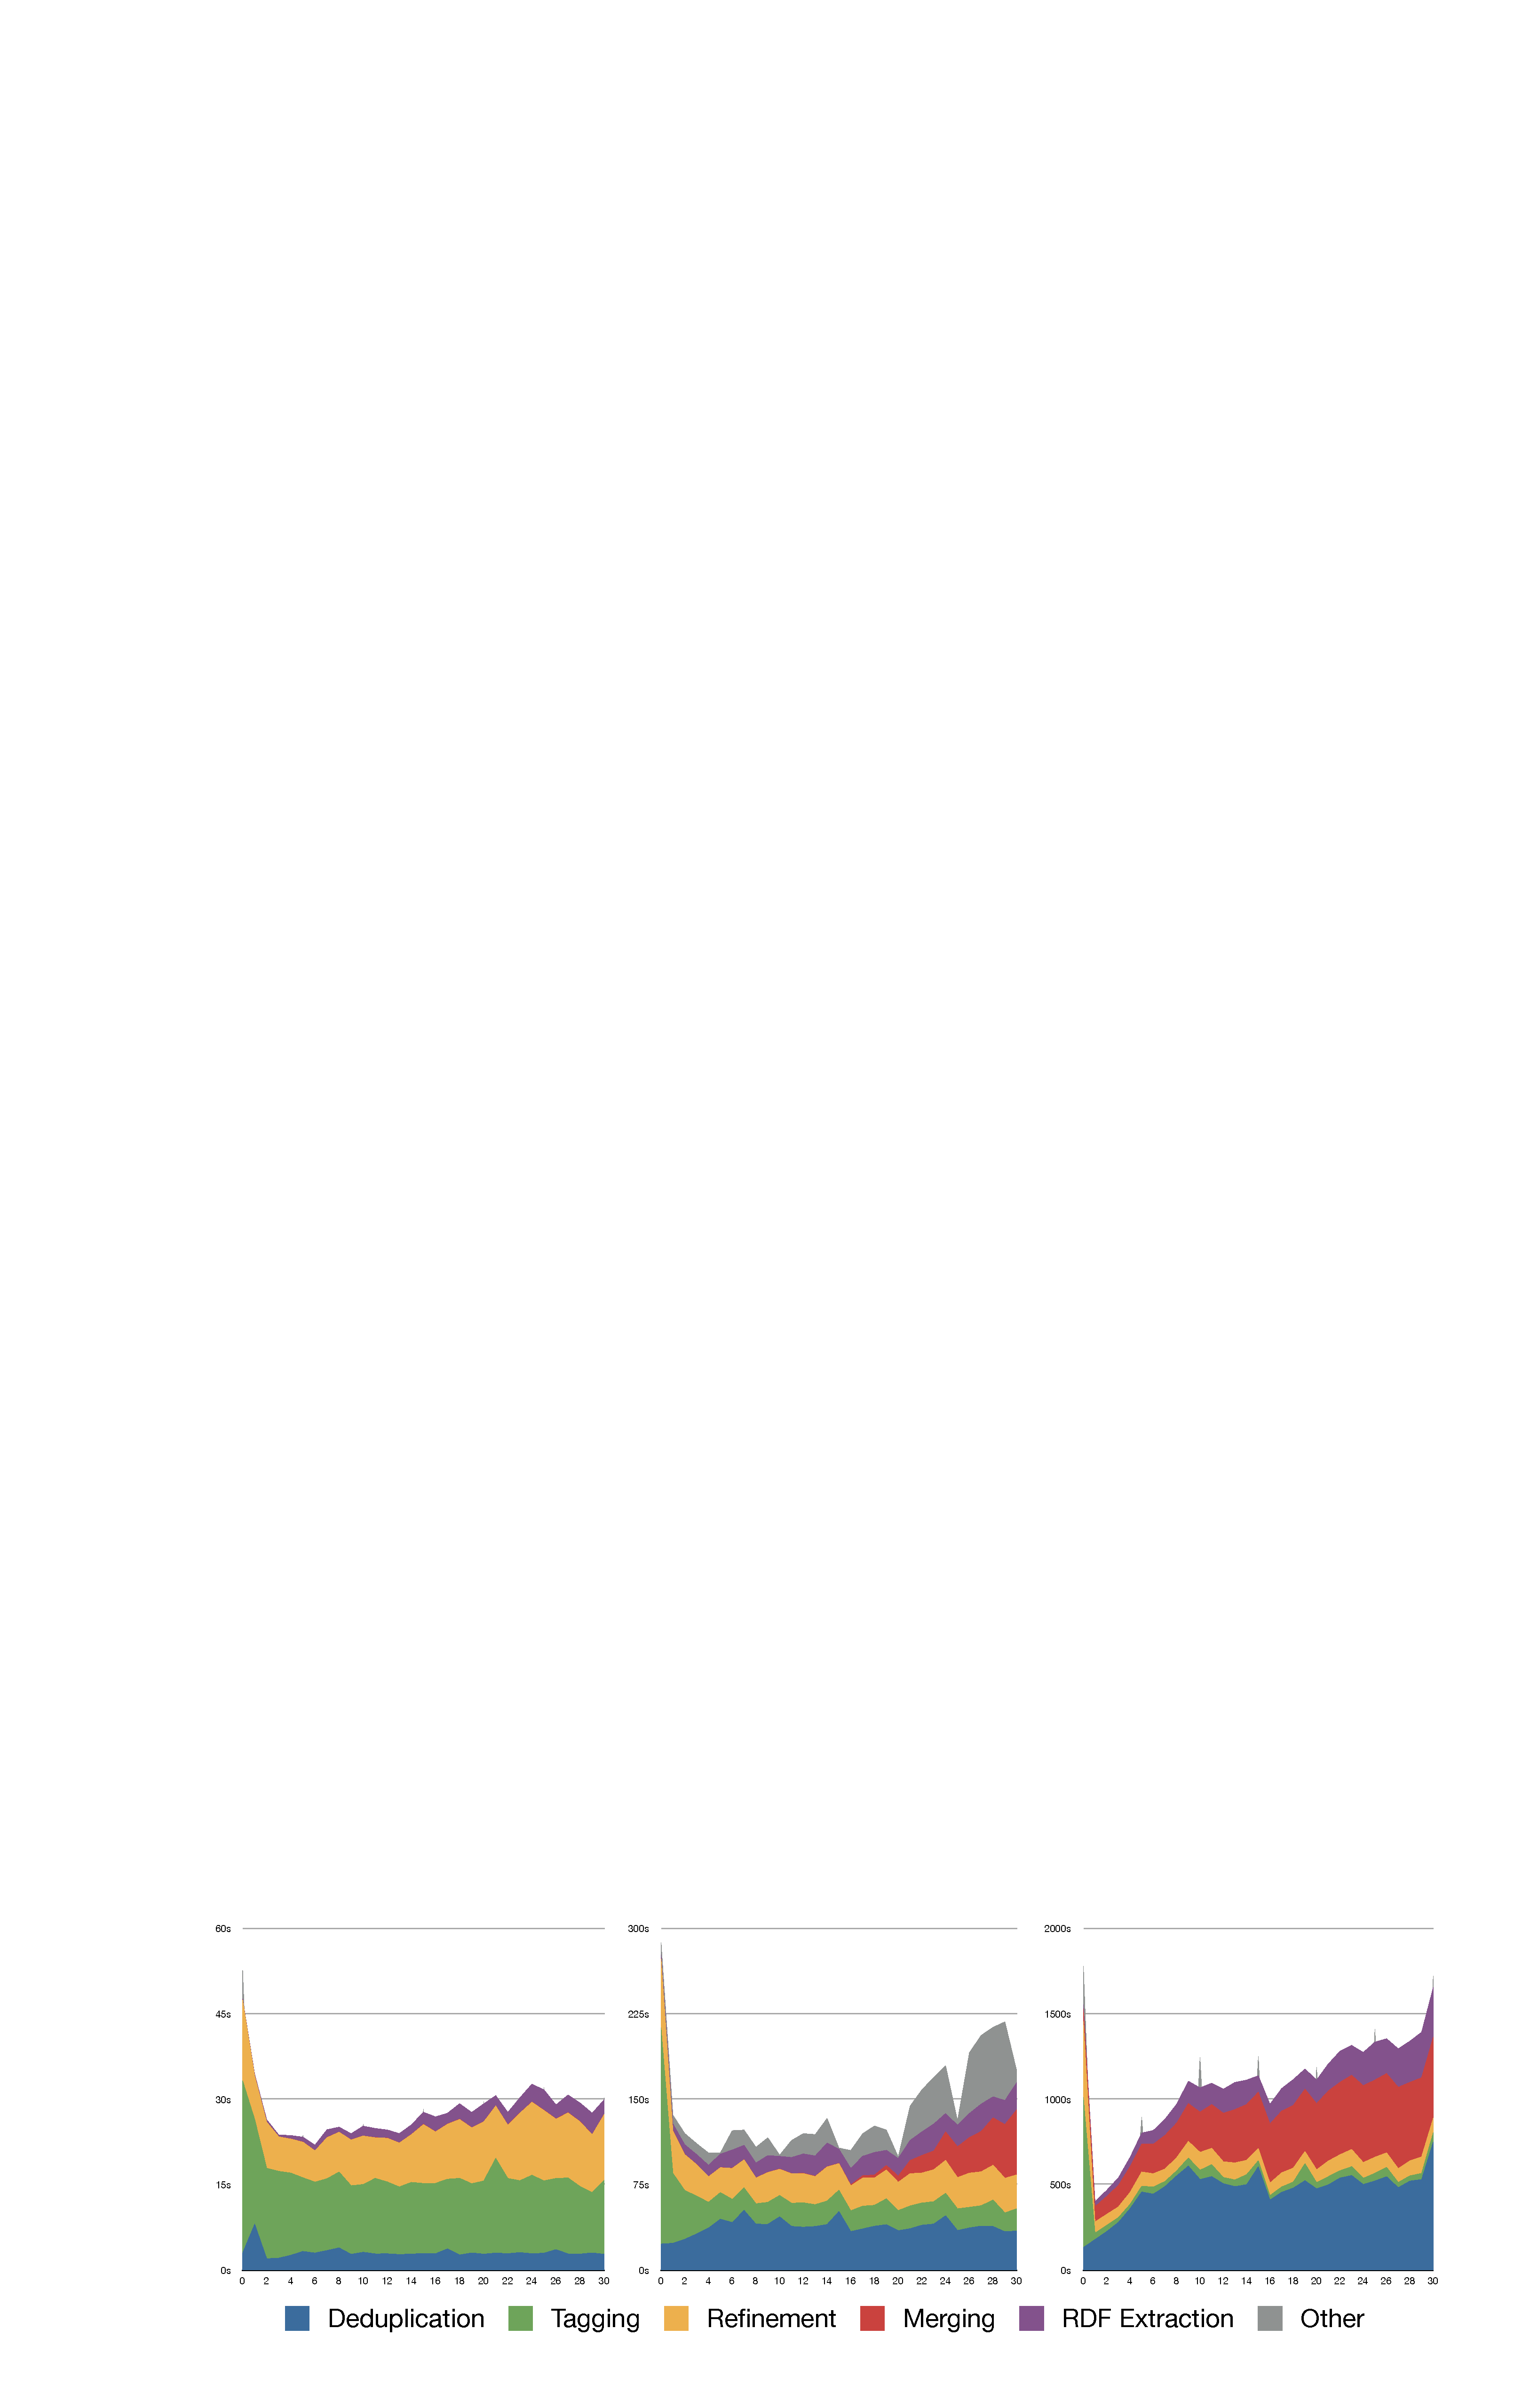
\includegraphics[width=\textwidth]{../images/speed.pdf}
    \end{block}
    \begin{itemize}
        \item Average time slice processing: 20min (2.2min for 10\%, 30s for 1\%) 
        \item Deduplication and merging largest bottlenecks
    \end{itemize}
\end{frame}

%------------------------------------------------

\begin{frame}
    \frametitle{Conclusion and Future Work}
    \begin{itemize}
		\item Presented RdfLiveNews, a framework for extraction of RDF from unstructured data streams
		\item URI disambiguation of 85\%, cluster patterns with accuracy of 82.5\% and achieve a total accuracy of about 90\%  
		\item Can handle 2h timeslices (300.000 sentences) in 20min
\pause
		\item Requires extension to support datatype properties
		\item Need for reification
		\begin{itemize}
	   		\item “\dots , Google said Motorola Mobility contributed revenue of
US\$ 1.25 billion for the second quarter.”		
    	\end{itemize}
		\item Integrate support for temporal logics
    \end{itemize}
\end{frame}

\begin{frame}{}
\begin{center}
\vspace{2cm}
\Huge{Thank you!}

\Huge{Questions?}
\end{center}

\begin{flushright}
Axel Ngonga \\
University of Leipzig \\
AKSW Research Group \\
Augustusplatz 10, Room P616 \\
04109 Leipzig, Germany \\
ngonga@informatik.uni-leipzig.de
\end{flushright}

\end{frame}
\end{document} 